\documentclass[crop,border=5pt,multi=tikzpicture]{standalone}
\usepackage{pgfplots}
\usepgfplotslibrary{groupplots,fillbetween}
\usepackage{animate}

\usepackage{pgf}
\usepackage{tikz}

\usetikzlibrary{fit}
\usetikzlibrary{positioning}
\usetikzlibrary{arrows}
\usetikzlibrary{automata}
\usetikzlibrary{backgrounds}
\usetikzlibrary{shapes.misc}

\usepackage{mathtools}
\usepackage{physics}


\usepackage{etoolbox}
\AtBeginEnvironment{quote}{\small}

\usepackage{float,color}
\usepackage{xcolor}
\definecolor{darkspringgreen}{rgb}{0.09, 0.45, 0.27}

\usepackage{tikz-qtree}
\usetikzlibrary{trees}

\begin{document}    

%%%%%%%%%%%%%%%%%%%%%%%%%%%%%%%%%%%
%% State variable diagram for KR82
%%%%%%%%%%%%%%%%%%%%%%%%%%%%%%%%%%% 

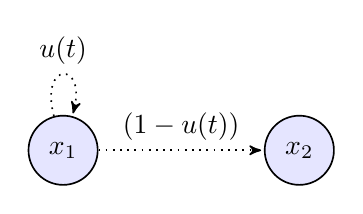
\begin{tikzpicture}[->,>=stealth',shorten >=1pt,auto,node distance=3cm,
            semithick]
\tikzstyle{every state}=[fill=blue!10,draw]    

\node [state] (a) { $x_1$ };
\node [state] (c) [right of=a] {$x_2$};
\path[dotted, ->] (a) edge node {$(1-u(t))$} (c);
\path[dotted] (a) edge [loop above] node {$u(t)$} (a);
\end{tikzpicture}

%%%%%%%%%%%%%%%%%%%%%%%%%%%%%%%%%%%
%% State variable diagrams for plants with determinate inflorescences
%%%%%%%%%%%%%%%%%%%%%%%%%%%%%%%%%%% 

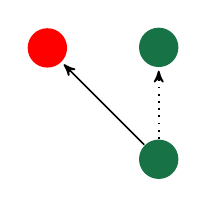
\begin{tikzpicture}[->,>=stealth',shorten >=1pt,auto,node distance=2cm, semithick]

\tikzstyle{every state}=[draw=none]

\node[state, fill=darkspringgreen,minimum size=.5cm] 	     (A)                    {};
\node[state, fill=red,minimum size=.5cm]         (B) [above left of=A] {};
\node[state, fill=darkspringgreen,minimum size=.5cm] 	     (D) [above = .9cm of A]                   {};
\path[dotted] (A) edge              (D);
\path[->] (A) edge (B);

\end{tikzpicture}

% split

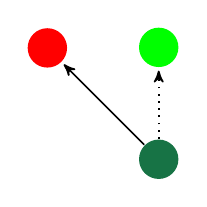
\begin{tikzpicture}[->,>=stealth',shorten >=1pt,auto,node distance=2cm, semithick]

\tikzstyle{every state}=[draw=none]

\node[state, fill = darkspringgreen,minimum size=.5cm] (A)                    {};
\node[state, fill = red,minimum size=.5cm]         (B) [above left of=A] {};
\node[state, fill=green,minimum size=.5cm] 	     (D) [above =.9cm of A]                   {};
\path[dotted] (A) edge              (D);
\path[->] (A) edge (B);

\end{tikzpicture}

% split

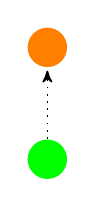
\begin{tikzpicture}[->,>=stealth',shorten >=1pt,auto,node distance=2cm, semithick]

\tikzstyle{every state}=[draw=none]

\node[state, fill = green,minimum size=.5cm] (A)                    {};
\node[state, fill = orange,minimum size=.5cm]         (C) [above =.9cm of A] {};
\path[dotted] (A) edge              (C);

\end{tikzpicture}

%%%%%%%%%%%%%%%%%%%%%%%%%%%%%%%%%%%
%% State variable diagrams for plants with branching and determinate inflorescences
%%%%%%%%%%%%%%%%%%%%%%%%%%%%%%%%%%% 

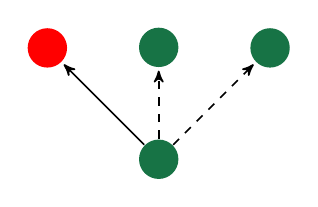
\begin{tikzpicture}[->,>=stealth',shorten >=1pt,auto,node distance=2cm,semithick]
                
\tikzstyle{every state}=[draw=none]

\node[state, fill=darkspringgreen,minimum size=.5cm] 	     (A)                    {};
\node[state, fill=red,minimum size=.5cm]         (B) [above left of=A] {};
\node[state, fill=darkspringgreen,minimum size=.5cm]         (C) [above right of=A] {};
\node[state, fill=darkspringgreen,minimum size=.5cm] 	     (D) [above = .9cm of A]                   {};

\path[dashed] (A) edge              (D)
        	edge               (C);
\path[->] (A) edge (B);

  \end{tikzpicture}

% split

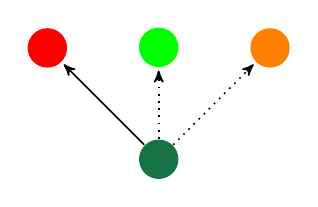
\begin{tikzpicture}[->,>=stealth',shorten >=1pt,auto,node distance=2cm,semithick]

\tikzstyle{every state}=[draw=none]

\node[state, fill = darkspringgreen,minimum size=.5cm] (A)                    {};
\node[state, fill = red,minimum size=.5cm]         (B) [above left of=A] {};
\node[state, fill = orange,minimum size=.5cm]         (C) [above right of=A] {};
\node[state, fill=green,minimum size=.5cm] 	     (D) [above =.9cm of A]                   {};

\path[dotted] (A) edge              (D)
        	edge               (C);
\path[->] (A) edge (B);

  \end{tikzpicture}

% split

  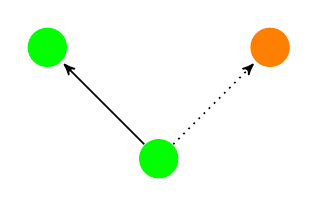
\begin{tikzpicture}[->,>=stealth',shorten >=1pt,auto,node distance=2cm,
                semithick]
                
\tikzstyle{every state}=[draw=none]

\node[state, fill = green,minimum size=.5cm] (A)                    {};
\node[state, fill = green,minimum size=.5cm]         (B) [above left of=A] {};
\node[state, fill = orange,minimum size=.5cm]         (C) [above right of=A] {};

\path[dotted] (A) edge              (C);
\path (A) edge		     (B);

  \end{tikzpicture}

\end{document}